% !TeX root = ../Main/XMU.tex
\chapter{基于深度学习的逆向运动学解算器及其应用}{Deep Inverse Kinematics Solver and Its Applications}
在本节中,将会完整阐述本文提出的基于监督学习方法的IK解算器。

\cref{fig:flowchart}说明了我们方法的整体流程。 CMU的动作捕捉库中的BVH文件是训练集和测试集的来源。在MATLAB中,对BVH文件进行解析和整合后,提取出神经网络的训练集和测试集。训练集和测试集一共三组,分别对应$\mathbf{MP}$和$\mathbf{PE}$和去噪滤波器(具体定义见\ref{sec:components}),六个文件,总大小超过$10$GB。$\mathbf{MP}$和$\mathbf{PE}$训练后,通过预先训练好的去噪滤波器,进一步对预测的姿态进行修正,得到最终结果。具体应用$\mathbf{IK}$解算器时,输入的轨迹(向量序列)依次经过$\mathbf{MP}$和$\mathbf{PE}$和去噪滤波器,得到最终的预测姿态。

本文方法的关键组件是Motion Predictor(MP)和Posture Estimator(PE)。前者根据当前运动轨迹来预测末端效应器的未来位置,而后者基于一系列末端效应器位置估计身体姿势。同时加入了去噪滤波器对网络的原始输出姿态进行修正,在很大程度上使预测的姿态更自然、更流畅。
\begin{figure}[!h]
	\centering
	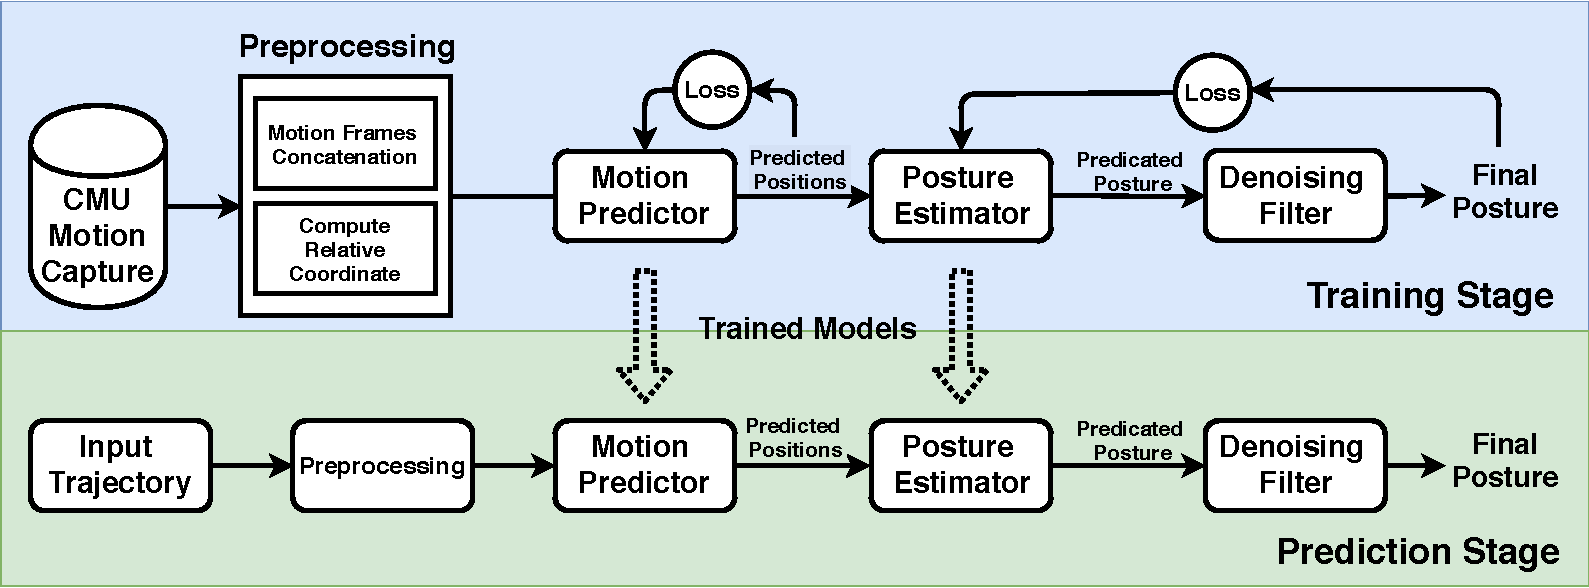
\includegraphics[width=\linewidth]{flowchart}
	\caption[]{\label{fig:flowchart}
		本方法的流程图
	}
\end{figure}

首先对本文中使用的一些术语进行定义:
\begin{itemize}
	\label{item:identify}
\item\textbf{骨骼(skelton)}骨骼$\mathbf{S}$定义具有根关节及其相互连接的关节角色的层次结构,而关节距离适用于构造具有几何变量的角色。
\item\textbf{末端执行器(end-effector)}末端执行器$\mathbf{EE}$通常指与环境进行交互的角色的脚和手。
\item\textbf{姿态(posture)}姿态$\mathbf{P}$是描述角色身体结构的向量,由根关节的全局变换和关节方向的角度值组成。
\item\textbf{动作(motion)}动作$\mathbf{M}$是一个矩阵,用于描述时域中的一系列角色姿势。矩阵行数对应帧数,列数与关节通道数成比例。
\item\textbf{位置(position)}位置$\mathbf{PE}$描述$\mathbf{EE}$的全局位置。
\end{itemize}

\section{离线网络学习}{Offline Network Learning}
\subsection{数据集和预处理}{Datasets and Preprocessing}
本次毕业论文使用Carnegie Mellon University(CMU)的Mocap数据库来构建此问题中的神经网络的训练集和测试集。 训练数据集包含约2000个动作序列(约200万个骨骼姿势),而测试数据集包含约200个动作序列(约20万个骨骼姿势)。运用MATLAB构建训练集和测试集时,使用正向运动学技术来计算骨骼关节的世界坐标位置。 我们提出了一种分层结构,将人体的四肢假设为互相独立的。所以整个人体姿态预测可以由四个独立的IK解算器组成,分别用于计算左/右臂和左/右腿。

我们定义了两种有效的技巧用来提高神经网络的学习性能:

\textbf{建立连续帧之间的时间关联性}过往的实验中,在解决\textbf{IK}问题时,往往只是将其归类为一个复杂的数学问题,忽视了它也是一个运动学问题,具备一定的时间关联性。实验证明,将连续的多帧的运动序列$[\cdots, X_{t-2*k}, X_{t-k},$ $ X_{t}, X_{t+k}, X_{t+2*k},\cdots]$替代传统的以末端执行器的当前位置作为网络输入在提高预测精度方面是有效的。 这在我们的实验中得到了证实(见\cref{fig:comparison_num_inputs}和章节\ref{sec:different_nums})。

\textbf{运用肩关节-腕关节/髋关节-踝节的相对坐标}在本次毕业论文中,通过计算肩关节-腕关节和髋关节-踝关节的相对向量来表示手臂和腿部的末端效应器的当前位置。采取这样的近似处理基于以下假设:股骨:胫骨和肱骨:尺骨的比例在个体之间的差异非常小。越来越多的研究表明,人虽然在身高和体重上的差别巨大,但是骨骼的比例确相差不多。而这样的处理也允许训练完毕后的IK解算器能够适应具有不同几何长度和几何形状的的角色,即无需得到待解决角色的肢体长度,也能预测出符合自然动作和流畅的姿态序列,这在以往的研究中是不存在的。

通过这些技巧,我们可以构建神经网络监督学习中\*X和\*Y之间的映射:

\begin{itemize}
\item $\mathbf{X}$:向量$N_X$表示从分层骨骼结构和动作联合通道中帧序列中末端效应器的全局位置。
\item $\mathbf{Y}$:向量$N_Y$表示身体各个关节方向的旋转角度值(BVH文件中角度的定义为欧拉角)。训练集和测试集中的该值直接从动作文件的相应通道进行复制。后续的操作中,为了提高神经网络的训练过程的表现,防止深层神经网络出现梯度爆炸、梯度消失等情况,对该值做了数学方法的处理(标准化),但不改变该值的原始定义和所表达的意义。
\end{itemize}

\subsection{IK解算器关键组件}{Main Components of IK Solver}
\label{sec:components}
Motion Predictor($\mathbf{MP}$)和Posture Estimator($\mathbf{PE}$)MP和PE是我们IK解算器的两个主要组成部分,我们使用大致相同的神经网络结构来构建这两个组件(需要指出,网络的输入输出是不同的)。 该网络的隐藏层是递归神经网络(RNN),具有三层LSTM(每层的大小为512),输入层和输出层是全连接层。

\begin{figure}[!h]
	\centering
	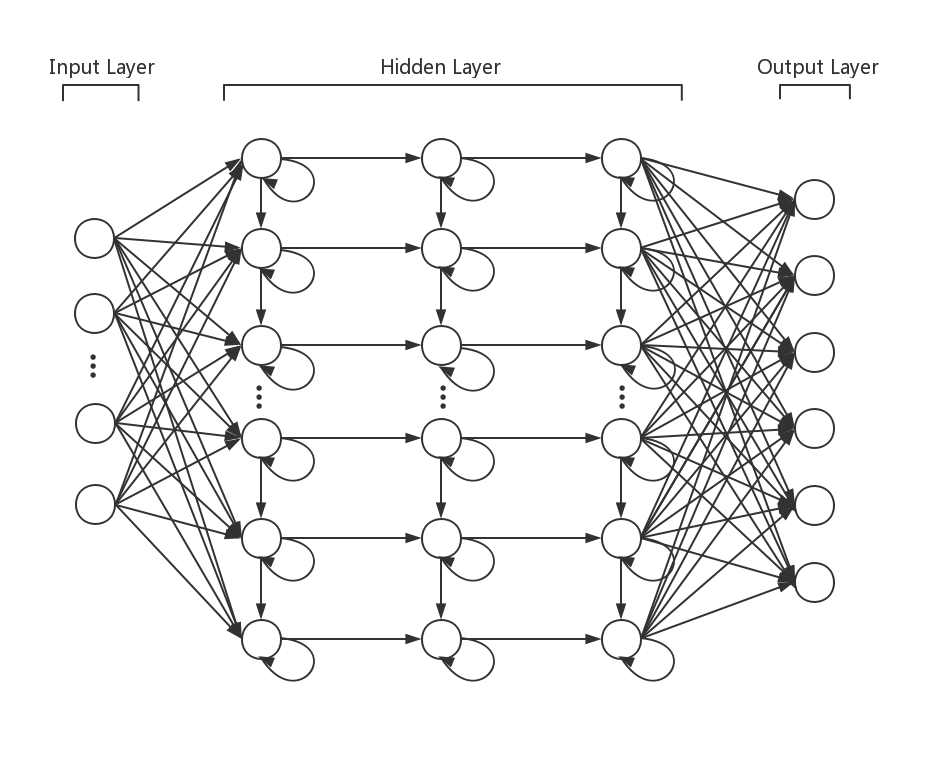
\includegraphics[width=0.8\linewidth]{network_mp}
	\caption[]{\label{fig:network_mp}
	$\mathbf{MP}$组件的网络结构
	}
\end{figure}
\paragraph{$\mathbf{MP}$网络结构}\cref{fig:network_mp}说明了$\mathbf{MP}$组件所用的神经网络的网络结构,该网络的输入是过去$\mathbf{K}$帧中的$\mathbf{EE}$位置序列,输出是下一个$\mathbf{K}$帧中的$\mathbf{EE}$位置序列。具体实现时,输入的帧数为$3$帧。设当前帧为第$i$帧,输入为第$i-10$帧、第$i-5$帧和第$i$帧。输入层有9个节点,分别表示输入帧各自的相对向量。输出的帧数为$2$帧。设当前帧为第$i$帧,输出为第$i+5$帧和第$i+10$帧。输出层共6个节点,分别表示输出帧各自的相对向量。将输入的帧数和输出的帧数进行整合后是$\mathbf{PE}$的输入。
\paragraph{$\mathbf{MP}$损失函数}

该神经网络的损失函数定义为:
\begin{equation}
L_m = \sum_{i=0}^{K_m} (\mathbf{PE}_i - \mathbf{PE}_i^G)
\end{equation}
该式中,$K_m$表示连续帧的帧数,$\mathbf{PE}_i^G$表示来自运动捕捉数据库的真实值.

\begin{figure}[!h]
	\centering
	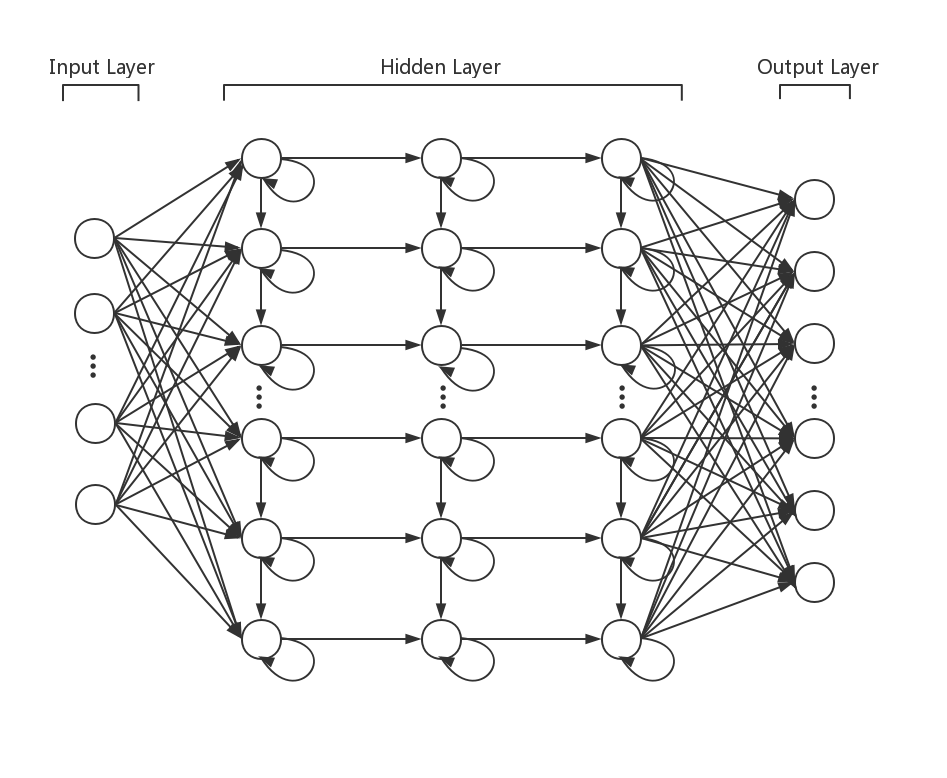
\includegraphics[width=0.8\linewidth]{network_pe}
	\caption[]{\label{fig:network_pe}
	$\mathbf{PE}$组件的网络结构
	}
\end{figure}

\paragraph{$\mathbf{PE}$网络结构}
\cref{fig:network_pe}说明了$\mathbf{PE}$组件所用的神经网络的网络结构,该网络的输入是过去$\mathbf{K}$帧中、当前帧和下一个$\mathbf{K}$帧中的位置序列,输出是过去当前帧和下一个$\mathbf{K}$帧中的$\mathbf{EE}$预测姿势序列。 具体实现时(以右手臂为例),输入的帧数为5帧。设当前帧为第$i$帧,输入的帧为第$i-10$帧、第$i-5$帧、第$i$帧和$\mathbf{MP}$输出的第$i+5$帧和第$i+10$帧,即将$\mathbf{MP}$
的输入和输出进行整合。输入层有15个节点,分别表示输入帧的各自相对向量。输出的帧数为$6$帧。设当前帧为第$i$帧,输出的帧为第$i$帧、第$i+1$帧、第$i+2$帧、第$i+3$帧、第$i+4$帧、第$i+5$帧。输出层有36个节点,,分别表示输出帧各自的肩关节和肘关节的旋转角。
\paragraph{$\mathbf{PE}$损失函数}
神经网络的损失函数定义为:
\begin{equation}
L_p = \sum_{i=0}^{K_p} (\mathbf{P}_i - \mathbf{P}_i^G)
\end{equation}
该式中,$K_p$表示连续帧的帧数,$\mathbf{P}_i^G$表示来自运动捕捉数据库的真实值。

\paragraph{激活函数、优化器和超参数}深度神经网络采用目前流行的RNN网络模型作为网络连接模式以适用连续帧之间的时间关联性,具体细节如下:
\begin{itemize}
	\item 选用线性整流函数(Rectified Linear Unit, ReLU)作为激活函数。线性整流函数定义了该神经元在线性变换$\mathbf{w}^{T} \mathbf{x}+b$之后的非线性输出结果。更加直观的理解为,对于来自上一层神经网络的输入向量$x$,该函数的神经元会输出$\max \left(0, \mathbf{w}^{T} \mathbf{x}+b\right)$。下一层神经元以此作为本层神经网络的输入。
	\item 选用Adam优化器作为优化函数。Adam结合AdaGrad和RMSProp两种优化算法的优点,对梯度的一阶矩估计(First Moment Estimation,即梯度的均值)和二阶矩估计(Second Moment Estimation,即梯度的未中心化的方差)进行综合考虑,计算出更新步长。更新规则如下:
	\begin{itemize}
		\item 计算时间梯度:$g_{t}=\nabla_{\theta} J\left(\theta_{\mathrm{t}-1}\right)$。
		\item 计算指数式的梯度移动的平均数,$\beta_1$为系数为指数衰减率,控制权重分配:$m_{t}=\beta_{1} m_{t-1}+\left(1-\beta_{1}\right) g_{t}$;$m_0$初始化为0。
		\item 计算梯度平方的指数移动平均数,$v_0$初始化为$0$。$\beta_2$系数为指数衰减率:$v_{t}=\beta_{2} v_{t-1}+\left(1-\beta_{2}\right) g_{t}^{2}$。
		\item 对梯度均值$m_t$进行偏差纠正,降低偏差对训练初期的影响:$\hat{m}_{t}=m_{t} /\left(1-\beta_{1}^{t}\right)$。
		\item 对$v_t$进行纠正:$\hat{v}_{t}=v_{t} /\left(1-\beta_{2}^{t}\right)$。
		\item 更新参数,初始的学习率$x$乘以梯度均值与梯度方差的平方根之比:$\theta_{\mathrm{t}}=\theta_{t-1}-\alpha^{*} \hat{m}_{t} /\left(\sqrt{\hat{v}_{t}}+\varepsilon\right)$。
	\end{itemize}
	\item 设置$batch size=128$,$learning_rate=0.0001$,$maximal epoch = 1000$。
\end{itemize}

\paragraph{网络参数调节}
在实际的训练过程中,为达到最好的训练效果,在模型的参数上和样本集的处理可能会做一些微调以达到更好的精度和更快的训练速度:
\begin{itemize}
\item{学习率自下降(learning rate adaptive decay)}防止学习率过大,在收敛到全局最优点的时候会来回摆荡,所以学习率随着训练轮数不断按指数级下降,收敛梯度下降的学习步长。

\item{梯度剪切(weithts regularization)}训练集的规模的约束导致了神经网络的层数在设计过程中需要比过往经验中的更多。正因如此,梯度爆炸和梯度消失的现象有可能在网络模型的参数调整过程中出现。为了解决这一问题,设计一个梯度阈值,如果超过该阈值,直接将梯度置为该值。
\end{itemize}

\subsection{去噪滤波器}{Denoising Filter}
\paragraph{平滑度}
合成动作的平滑度是IK技术成功与否的关键衡量标准之一\cite{aristidou2018inverse},特别是在一些涉及收敛的迭代算法中。通常,建议程序在固定的迭代次数之后终止循环以避免程序陷入无限循环。 然而,这个操作可能只能得到次优结果并导致合成动作的波动。
\paragraph{自然度}
评估一个动作序列是否是自然的是困难的因为它没有一个固定的标准,除此之外,这个标准可能根据不同的场景和主题而随之变化。本次毕业论文中,在自然度的评估是通过比较合成动作和原始动作数据之间的差异,差异越小则代表动作越自然。之所以能做出这样的标准是因为本文采用的动作数据来自真实的人体动作捕捉,并非通过计算机模拟产生。
\textbf{PE}网络的输出存在一定的噪音(连续帧之间动作不够平滑和自然,更直观的说法为视觉上骨骼轻微抖动)进一步使用平均滤波器进行处理以进行去噪。平均滤波器的处理过程如下:
\begin{equation}
	\label{equ:filter}
\mathbf{P} = \frac{1}{N} (\sum_i^{i+k} {\mathbf{P}_i}+\sum_{i-k}^i{\mathbf{P}_j})
\end{equation}
$\mathbf{P}_i$表示\textbf{PE}网络输出的连续预测姿势序列,$\mathbf{P_j}$表示由内存中读取的过往姿势序列。

具体实现中,设当前帧为第$x$帧,\ref{equ:filter}中$i=x-5$,$k=x+5$。从第$x-5$帧至第$x-1$帧为已知,因为是过往姿势序列,可以从内存中直接读取;从第$x$帧到第$x+5$帧为$\mathbf{PE}$网络的输出。最终得到的$\mathbf{P}$为降噪后的姿势形态。
\label{sec:denoising}
这一步显著提高了\textbf{PE}输出预测姿势序列的平滑度,具体降噪效果见\ref{res:denoising}。

\section{姿势合成和姿势估计}{Posture Synthesis and Estimation}

本次毕业论文的IK求解器应用于两个应用:姿势合成和姿态估计。

\subsection{姿势合成}{Posture Synthesis}在用户指定末端执行器的轨迹后,即末端执行器在三维世界坐标内的位置序列,以0.5秒的均匀间隔对轨迹进行采样,然后运用$\mathbf{IK}$解算器自动生成全身姿势。轨迹的生成由两个步骤组成:相对坐标的计算和运动帧级联。相对坐标的计算指的是(以右手臂为例):捕捉右臂的肩关节、肘关节、腕关节的末端执行器的位置,以~\ref{sec:Retargetting}中所示方法计算出某一个时刻某一个姿势唯一的右臂向量;运动帧级联指的是在构造输入数据时,加入本文提出的连续帧之间的时间关联性,整合出符合训练好的解算器组件输入格式的数据。预测程序的流程如\cref{fig:flowchart}所示。
\begin{figure}[!h]
	\centering
	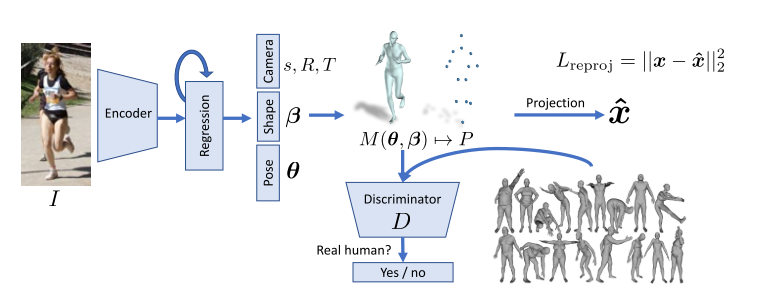
\includegraphics[width=\linewidth]{2dto3d}
	\caption[]{\label{fig:2dto3d}
	2D图像到3D人体骨骼预测流程\cite{kanazawa2018end}。
	}
\end{figure}输入的2D图像$I$首先通过$\mathbf{Encoder}$。$\mathbf{Encoder}$输出的结果传送到迭代$\mathbf{3D regression}$模块(该模块能够推断人的隐式三维表达方式来减少人体关节投影的误差)。3D参数也被发送到$\mathbf{Discriminator}$,鉴别器($\mathbf{Discriminator}$)$\mathbf{D}$的目的是告知这些参数是否来自真实的人体形状和姿势。
\subsection{姿态估计}{Posture Estimation}
本次毕业论文着重于改进使用单目摄像机捕捉图像到3D人体骨骼姿态的估计结果\cite{kanazawa2018end}。由于这是一个典型的不适定问题,所以解决该问题时具有一定的挑战性。

2D图像到3D人体骨骼的预测大致框架如\cref{fig:2dto3d}所示。涉及论文中提出直接利用以人为中心的单张RGB图像来重建人体完整的三维网格模型。神经网络训练过程中,假设所有图像都使用真实的二维关节进行注释,该方法还考虑了一些具有三维注释的情况。

除此之外,该方法假设有一个具有不同形状和姿势的人体三维网格池。由于这些网格不一定有相应的图像与之对应,因此我们将此数据称为未配对数据。\cref{fig:2dto3d}展示了所提出的预测网络架构。该网络可以执行端到端的训练。为了推断3D人体网格和相机,一张图像的卷积特征被发送到迭代3D回归模块,使得其3D关节投射到带注释的2D关节上。预测的人体参数传送到一个鉴别器网络。鉴别器的任务是确定3D参数是否是来自未配对数据。这步操作可以促进网络输出基于多样式人体形态的3D人体网格,并且能够作为没有真实3D注释的原始图像的弱监督。得益于3$L=\lambda\left(L_{\text { reproj }}+\mathbb{1} L_{3 \mathrm{D}}\right)+L_{\mathrm{adv}}$D网格模型具有多种表达方式,数据驱动先验方法可以捕获关节角度限制,人体测量约束(例如身高,体重,骨骼比率)。当拥有真实3D信息时,将其作为中间损失。总的来说,该方法的目标
\begin{equation}
	L=\lambda\left(L_{\text { reproj }}+\mathbb{1} L_{3 \mathrm{D}}\right)+L_{\mathrm{adv}}
\end{equation}其中$\lambada$控制每个物体的关联性的重要程度;$\mathbf{1}$是指示器函数,如果拥有真实值可用于图像则为1,否则为0。每个组件的具体实现如下:
\begin{itemize}
	\item \textbf{3D人体表达方式}该方法使用$\mathbf{SMPL}$模型来编码人体的3D网格
。形状参数$\boldsymbol{\beta} \in \mathbb{R}^{10}$由$\mathbf{PCA}$形状空间的前10个系数参数化得到。姿势参数$\boldsymbol{\theta} \in \mathbb{R}^{3 K}$$K = 23$个关节的相对3D旋转角来建模。 $\mathbf{SMPL}$是一个可微函数,它输出一个有$N=6980 $个顶点和
 $M(\boldsymbol{\theta}, \boldsymbol{\beta}) \in \mathbb{R}^{3 \times N}$ 的三角网格。通过线性回归得到的3D关键点($X(\boldsymbol{\theta}, \boldsymbol{\beta}) \in \mathbb{R}^{3 \times P}$)可以用于计算投影误差。
 \item \textbf{带回馈3D交互回归}3D回归模块的目标是输出带图像编码$\phi$的$\Theta$
使得联合重投影误差$L_{\text { reproj }}=\Sigma_{i}\left\|v_{i}\left(\mathbf{x}_{i}-\hat{\mathbf{x}}_{i}\right)\right\|_{1}$最小化。式中$\mathbf{x}_{i} \in \mathbb{R}^{2 \times K}$是第$i$个真实2D关节。$v_{i} \in\{0,1\}^{K}$是$K$个关节的各自是否可视化值。

3D回归模块将图像特征$\theta$和当前参数$\Theta_t$作为输入并输出残差$\Delta \Theta_{t}$。 通过将该残差加到当前估计$\Theta_{t+1}=\Theta_{t}+\Delta \Theta_{t}$来更新参数。 初始估计$\Theta_0$被设置为平均$\overline{\Theta}$。 以下是3D损失的定义:
\begin{equation}
\begin{aligned} L_{3 \mathrm{D}} &=L_{3 \mathrm{D} \text { joints }}+L_{3 \mathrm{D} \text { smpl }} \\ L_{\text { joints }} &=\left\|\left(\mathbf{X}_{\mathbf{i}}-\hat{\mathbf{X}}_{\mathbf{i}}\right)\right\|_{2}^{2} \\ L_{\text { smpl }} &=\left\|\left[\boldsymbol{\beta}_{i}, \boldsymbol{\theta}_{i}\right]-\left[\hat{\boldsymbol{\beta}}_{i}, \hat{\boldsymbol{\theta}}_{i}\right]\right\|_{2}^{2} \end{aligned}
\end{equation}
\item \textbf{分解对抗性先验}该工作使用经过训练的鉴别器网络$D$来判断$\mathbf{SMPL}$参数是否对应于人体真实值。将此称为对抗性先验,因为鉴别器充当引导3D预测的数据驱动先验。该方法镜像$\mathbf{SMPL}$的形状并进行了姿势分解,独立训练形状和姿势的鉴别器。因为姿势的预测基于动作树,所以进一步分解姿势鉴别器并单独为每个关节训练一个。为了捕获整个动作树的联合分布,训练一个接受所有旋转的鉴别器。由于每个鉴别器的输入是非常低的维度($\beta$为$10-D$,每个关节为$9-D$,所有关节为$9K-D$),因此训练的网络都可以是小型网络。所有姿势鉴别器共享旋转矩阵的共同特征空间,并且仅分别学习最终分类器。

在所有训练的$k+2$个鉴别器中,每个鉴别器$D_i$的输出介于$[0,1]$之间,用此来表示$\Theta$来自数据库的可能性。实际训练过程中,使用最小二乘法来保证其稳定性。设$E$表示包括图像编码器和3D模块的编码器。编码器的对抗性损失函数是:\begin{equation}
\min L_{\text { adv }}(E)=\sum \mathbb{E}_{\Theta \sim p_{E}}\left[\left(D_{i}(E(I))-1\right)^{2}\right]。
\end{equation}
每个鉴别器的目标是:\begin{equation}
\min L\left(D_{i}\right)=\mathbb{E}_{\Theta \sim p_{\text { data }}}\left[\left(D_{i}(\Theta)-1\right)^{2}\right]+\mathbb{E}_{\Theta \sim p_{E}}\left[D_{i}(E(I))^{2}\right]
\end{equation}
\end{itemize}


在实际的应用中,对于每个人体几何信息进行采集几乎是不可能的,所以本文所涉及的工作中,仅使用由2D图像到3D骨骼预测流程中输出的$\mathbf{EE}$的3D位置和与其对应的根关节位置,并应用本文提出的IK解算器对当前身体骨骼连接做出一个最佳姿态的估计。

\section{本章小结}{Summary}
在本节中,将会完整阐述本文提出的基于监督学习方法的IK解算器。

首次介绍了本文方法的完整流程,其次介绍了IK解算器的关键组件,包括MP、PE和去噪滤波器三个组件,并详细描述了了组件的网络结构和超参数等。

最后,完整地介绍了本文涉及方法的两个应用-姿势合成和姿态估计,并对姿态估计的方法做了完整的阐述。
